%% Template file for all Software/Hardware modules

% Replace "Name of Module" with the name of this module
\subsection{Measurement Hardware}
Current and voltage running through the mains outlet to the Satellite's associated device must be measured and sent to the Server. 
The measuring circuit, shown in figure \ref{MeasureCircuit}, costists of the following parts:

\begin{itemize}
	\item Current transformer
	\item Diode
	\item .1 Ohm sense-resistor
\end{itemize}

The current transformer acts as a middle man between the outlet and it's attached device. 
A step-down current transformer will be used to take a fraction of the current, equal to the ratio of the transformer. 
Since we're dealing with Alternating Current (AC) voltage, there will parts of the waveform that are negative. 
To rule out the negative half-cycles, the current sample will pass through a diode. 
After the current passes through a diode, it will be passed through a sense-resistor, and then into an Analog to Digital Converter (ADC) pin on the interface board. 
The sense-resistor is in place to make measuring, verifying and troubleshooting the circuit a little easier. 

\begin{figure}[H]
\centering
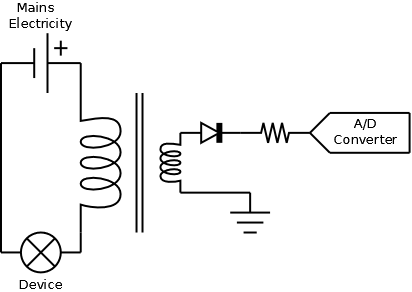
\includegraphics[scale=0.3]{Hardware/images/MeasureCircuit.png}
\caption{Wiring Schematic for Measuring Current}
\label{MeasureCircuit}
\end{figure}
